% Figura cuerpo B1: las elasticidades de la Síntesis: IS inelástica, LM elástica, y la lectura de las dos políticas
\documentclass[tikz,border=3pt]{standalone}
\usepackage[T1]{fontenc}
\usepackage[utf8]{inputenc}
\usetikzlibrary{arrows.meta,calc,positioning}
\begin{document}
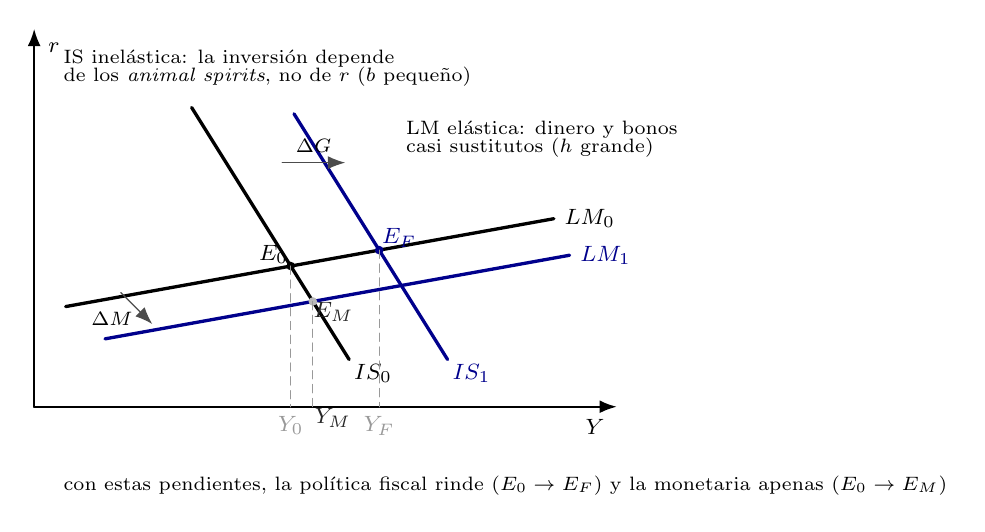
\begin{tikzpicture}[>={Latex[length=2.2mm]}, line cap=round, font=\footnotesize,
  eje/.style={->, thick},
  curva/.style={very thick},
  nueva/.style={very thick, blue!55!black},
  guia/.style={densely dashed, gray!80},
  pto/.style={circle, fill=black, inner sep=1.1pt}]
  \draw[eje] (0,0) -- (7.4,0) node[below left=1pt]{$Y$};
  \draw[eje] (0,0) -- (0,4.8) node[below right=2pt]{$r$};
  % LM plana (h grande) y LM' (politica monetaria)
  \draw[curva] (0.4,1.272) -- (6.6,2.388) node[right]{$LM_0$};
  \draw[nueva] (0.9,0.862) -- (6.8,1.924) node[right]{$LM_1$};
  % IS empinada (b pequeño) e IS' (politica fiscal)
  \draw[curva] (2.0,3.8) -- (4.0,0.6) node[below right=-3pt]{$IS_0$};
  \draw[nueva] (3.3,3.72) -- (5.25,0.6) node[below right=-3pt]{$IS_1$};
  \draw[->, gray!60!black] (3.15,3.1) -- (3.95,3.1) node[midway, above=0pt, black]{\scriptsize $\Delta G$};
  \draw[->, gray!60!black] (1.1,1.45) -- (1.5,1.05) node[midway, below left=-3pt, black]{\scriptsize $\Delta M$};
  % Equilibrios
  \node[pto] (E0) at (3.258,1.787) {};
  \node[above left=-2pt of E0, inner sep=1pt] {$E_0$};
  \node[pto, fill=blue!55!black] (EF) at (4.382,1.989) {};
  \node[above right=-2pt of EF, inner sep=1pt, blue!55!black] {$E_F$};
  \node[pto, fill=gray!55] (EM) at (3.539,1.337) {};
  \node[below right=-3pt of EM, inner sep=1pt, gray!30!black] {$E_M$};
  \draw[guia] (3.258,1.787) -- (3.258,0) node[below]{$Y_0$};
  \draw[guia] (3.539,1.337) -- (3.539,0) node[below right=-4pt, gray!30!black]{$Y_M$};
  \draw[guia] (4.382,1.989) -- (4.382,0) node[below]{$Y_F$};
  % Anotaciones de creencias
  \node[align=left, anchor=north west] at (0.25,4.65) {\scriptsize IS inelástica: la inversión depende\\[-3pt]\scriptsize de los \textit{animal spirits}, no de $r$ ($b$ pequeño)};
  \node[align=left, anchor=west] at (4.6,3.4) {\scriptsize LM elástica: dinero y bonos\\[-3pt]\scriptsize casi sustitutos ($h$ grande)};
  \node[align=left, anchor=north west] at (0.25,-0.75) {\scriptsize con estas pendientes, la política fiscal rinde ($E_0\to E_F$) y la monetaria apenas ($E_0\to E_M$)};
\end{tikzpicture}
\end{document}
